\section{Auswertung}
\label{sec:Auswertung}


\subsection{Bestimmung der Zeitkonstante}
Die Werte, die für die Bestimmung der Zeitkonstante $RC$ nötig sind, befinden sich in Tabelle \ref{table: }. %Tabelle
%Hier Tabelle einfügen
\begin{table}\caption{Die Länge der Zylinder und die Spannung mit den jeweiligen Zeitenpunkten der Ausschläge.}
\label{taba}
\centering
\sisetup{round-mode = places, round-precision=2, round-integer-to-decimal=true}
\begin{tabular}{S[]S[]S[]S[]S[]} 
\toprule
{$l/ \si{\milli\meter}$} & {$U_1/ \si{\volt}$} & {$t_1/ \si{\micro\second}$} & {$U_2/ \si{\volt}$} & {$t_2/ \si{\micro\second}$}\\
\midrule
120.8 & 1.29 & 0.6 & 0.17 & 88.7\\
102.3 & 1.27 & 0.5 & 0.2 & 76.5\\
80.5 & 1.33 & 0.6 & 0.76 & 59.8\\
40.4 & 1.33 & 0.5 & 1.34 & 30.2\\
31.1 & 1.29 & 0.5 & 1.37 & 23.8\\
\bottomrule
\end{tabular}\end{table}
\begin{table}\caption{Der zeitliche Verlauf $t$ gegen den negativen Logarithmus der Spannungswerte geteilt durch die maximale Spannung}
\label{taba}
\centering
\sisetup{round-mode = places, round-precision=5, round-integer-to-decimal=true}
\begin{tabular}{S[]S[]} 
\toprule
{$t/ \si{\second}$} & {$-log(\frac{U(t)}{U_{0}})$}\\
\midrule
0.0 & -0.0\\
0.0004 & 0.13372577497521726\\
0.0008 & 0.4281699018019215\\
0.0012 & 0.705467664947986\\
0.0016 & 0.9977516783331359\\
0.003 & 1.3015531326648002\\
0.0024 & 1.623136756792262\\
0.0028 & 1.8993901334204206\\
0.0032 & 2.2178438645389553\\
0.0036 & 2.505525936990737\\
0.004 & 2.793208009442516\\
0.0044 & 3.19867311755068\\
0.0048 & 3.604138225658845\\
0.0052 & 4.29728540621879\\
0.0056 & 4.990432586778735\\
\bottomrule
\end{tabular}\end{table}
Die Zeitkonstante berechnet sich mittels Gleichung \eqref{eqn: RC} zu $RC = $. %Wert für RC 

\begin{figure}
  \centering
  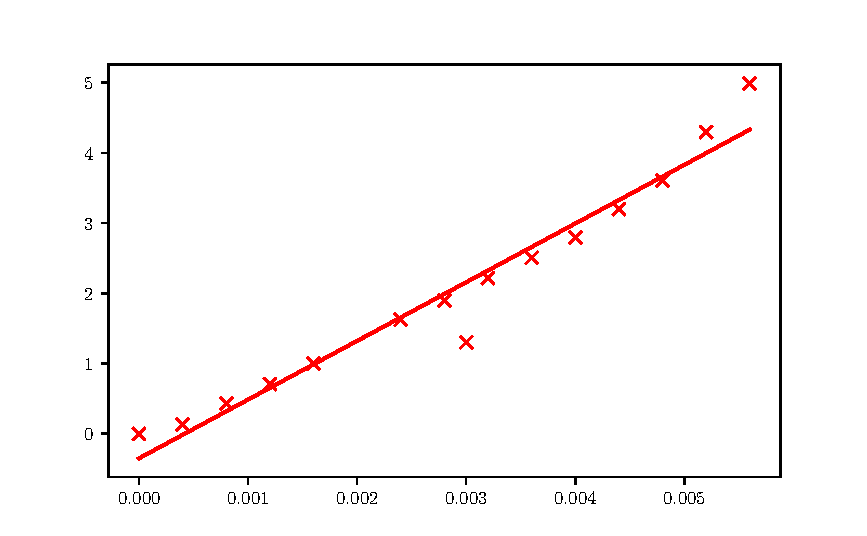
\includegraphics{build/plota.pdf}
  \caption{}
  \label{fig:plota}
\end{figure}

\subsection{4b}
Die Kondensatorspannungen in Abhängigkeit von der Frequenz sind in Tabelle \ref{table: } dargstellt. %Tabelle
%Hier Tabelle einfügen
\begin{table}\caption{Die angelegte Spannung des elektrischen Feldes innerhalb des Geiger-Müller-Zählrohrs, die Anzahl der jeweils gemessenen Impulse und der Strom innerhalb des Geiger-Müller-Zählrohrs.}
\label{tabb}
\centering
\sisetup{round-mode = places, round-precision=2, round-integer-to-decimal=true}
\begin{tabular}{c c S[]} 
\toprule
{$U / \si{\volt}$} & {$\frac{N}{\SI{130}{\second}}$} & {$I / \si{\ampere}$}\\
\midrule
320 & 11298 & 0.1\\
400 & 11820 & 0.2\\
480 & 12135 & 0.3\\
540 & 12301 & 0.35\\
560 & 12068 & 0.4\\
600 & 12354 & 0.45\\
640 & 12403 & 0.5\\
660 & 12507 & 0.55\\
680 & 12659 & 0.6\\
\bottomrule
\end{tabular}\end{table}
\begin{table}\caption{}
\label{}
\centering
\sisetup{round-mode = places, round-precision=2, round-integer-to-decimal=true}
\begin{tabular}{S[]S[]} 
\toprule
{$\frac{1}{\omega}/ \si{\second}$} & {$\sqrt{\frac{1}{\frac{U_{0}}{A(\omega)}^{2}-1}}$}\\
\midrule
0.0024485375860291594 & 2.262660907951623\\
0.0019894367886486917 & 1.7091833258800144\\
0.0015915494309189533 & 1.2706566931710195\\
0.0006366197723675814 & 0.48280454958526764\\
0.00039788735772973834 & 0.2991883988251616\\
0.0002448537586029159 & 0.18505403427568887\\
0.00019894367886486917 & 0.14980117725462763\\
0.00015915494309189535 & 0.14980117725462763\\
6.366197723675813e-05 & 0.0483656490240811\\
3.978873577297384e-05 & 0.030287634503871775\\
2.448537586029159e-05 & 0.01884392449684891\\
1.989436788648692e-05 & 0.015621873649013022\\
1.5915494309189534e-05 & 0.01240030915098555\\
\bottomrule
\end{tabular}\end{table}

Die Zeitkonstante wird wieder durch \eqref{eqn: RC} berechnet. Es ergibt sich $RC = $. %Wert für RC

\begin{figure}
  \centering
  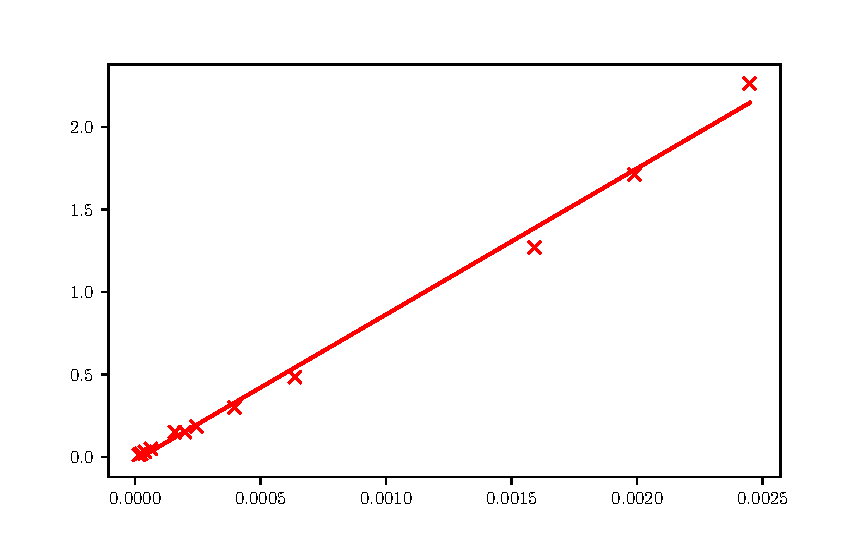
\includegraphics{build/plotb.pdf}
  \caption{}
  \label{fig:plotb}
\end{figure}

\subsection{4c}
In Tabelle \ref{table: } sind die Abstände der Nulldurchgänge der Spannung des Kondensators und der Spannung %Tabelle
des Generators in Abhängigkeit von der Frequenz dargestellt.
%Hier Tabelle einfügen
\begin{table}\caption{Der Anodenstrom und der Kathodenstrom bei einer Beschleunigungsspannung von $U_\text{B} = \SI{25}{\kilo\volt}$ und einer Kathodenspannung $U_\text{K,1} = \SI{500}{\volt}$ und einer Kathodenspannung $U_\text{K,2} = \SI{300}{\volt}$ bei einem Blendenradius von $r_\text{B} = \SI{5}{\milli\meter}$.}
\label{tabc}
\centering
\sisetup{round-mode = places, round-precision=2, round-integer-to-decimal=true}
\begin{tabular}{S[]S[]S[]} 
\toprule
{$I_\text{K} / \si{\milli\ampere}$} & {$I_\text{K,1} / \si{\nano\ampere}$} & {$I_\text{K,2} / \si{\nano\ampere}$}\\
\midrule
1.0 & 2.6 & 2.4\\
0.95 & 2.5 & 2.4\\
0.9 & 2.4 & 2.2\\
0.85 & 2.3 & 2.1\\
0.8 & 2.2 & 2.0\\
0.75 & 2.1 & 1.9\\
0.7 & 1.9 & 1.8\\
0.65 & 1.8 & 1.6\\
0.6 & 1.6 & 1.5\\
0.55 & 1.5 & 1.4\\
0.5 & 1.4 & 1.3\\
0.45 & 1.2 & 1.2\\
0.4 & 1.1 & 1.0\\
0.35 & 0.9 & 0.9\\
0.3 & 0.8 & 0.8\\
0.25 & 0.6 & 0.6\\
0.2 & 0.5 & 0.5\\
0.15 & 0.4 & 0.4\\
0.1 & 0.1 & 0.2\\
0.05 & 0.1 & 0.1\\
\bottomrule
\end{tabular}\end{table}
\begin{table}\caption{Der Kehrwert der Kreisfrequenz gegen den negativen Kehrwert des Tangens der Phase, die sich durch die negative Division der zeitlichen Phasenverschiebung durch die Periodendauer multipliziert mit \pi ergibt}
\label{tabc}
\centering
\sisetup{round-mode = places, round-precision=5, round-integer-to-decimal=true}
\begin{tabular}{S[]S[]} 
\toprule
{$\frac{1}{\omega}/ \si{\second}$} & {$-\frac{1}{tan(\phi(\omega))}$}\\
\midrule
0.0024485375860291594 & 3.117626187195526\\
0.0019894367886486917 & 2.723786837133246\\
0.0015915494309189533 & 2.2715973027329865\\
0.0006366197723675814 & 1.4714553158199692\\
0.00039788735772973834 & 1.2401991640705359\\
0.0002448537586029159 & 1.2010895549922853\\
0.00019894367886486917 & 1.120011792429241\\
0.00015915494309189535 & 1.0000000000000002\\
6.366197723675813e-05 & 0.8540806854634666\\
3.978873577297384e-05 & 1.0126459941540735\\
2.448537586029159e-05 & 1.0190294678742615\\
1.989436788648692e-05 & 1.064891840324792\\
1.5915494309189534e-05 & 1.064891840324792\\
\bottomrule
\end{tabular}\end{table}
Mittels \eqref{eqn: RC} berechnet sich die Zeitkonstante zu $RC = $. %Wert für RC

\begin{figure}
  \centering
  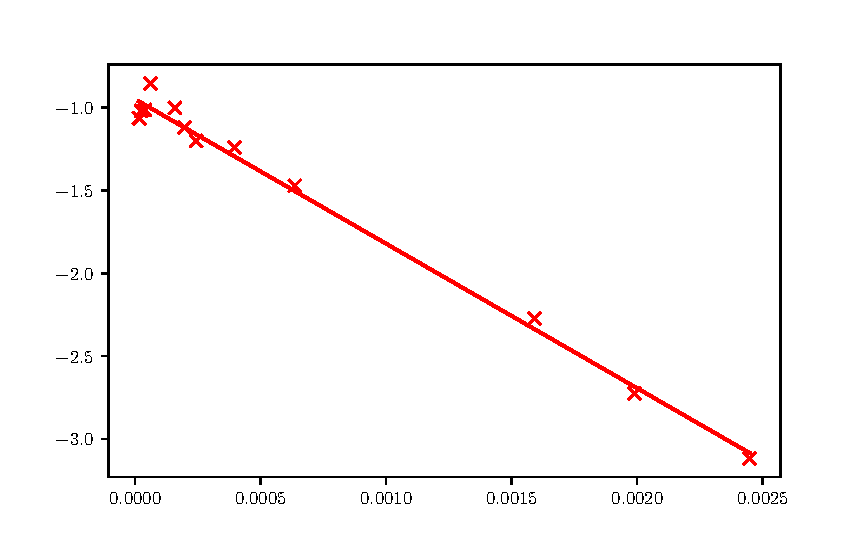
\includegraphics{build/plotc.pdf}
  \caption{}
  \label{fig:plotc}
\end{figure}

\subsection{4d}

%Tabellen
\begin{table}\caption{Die Phasenverschiebung gegen die Amplitude der Spannung $U_{C}$ geteilt durch die maximale Spannung $U_{0}}
\label{tabd}
\centering
\sisetup{round-mode = places, round-precision=5, round-integer-to-decimal=true}
\begin{tabular}{S[]S[]} 
\toprule
{$\phi/ \si{\radian}$} & {$\frac{A(\omega)}{U_{0}}$}\\
\midrule
-0.31038935417467156 & 0.9146537842190016\\
-0.3518583772020568 & 0.8631239935587762\\
-0.4146902302738527 & 0.7858293075684379\\
-0.5969026041820606 & 0.4347826086956522\\
-0.6785840131753953 & 0.286634460547504\\
-0.6942919764433444 & 0.1819645732689211\\
-0.728849495632832 & 0.14814814814814814\\
-0.7853981633974483 & 0.14814814814814814\\
-0.8639379797371932 & 0.04830917874396135\\
-0.7791149780902686 & 0.03027375201288245\\
-0.7759733854366789 & 0.01884057971014493\\
-0.7539822368615503 & 0.015619967793880838\\
-0.7539822368615503 & 0.012399355877616747\\
\bottomrule
\end{tabular}\end{table}

%Plots einfügen
\begin{figure}
  \centering
  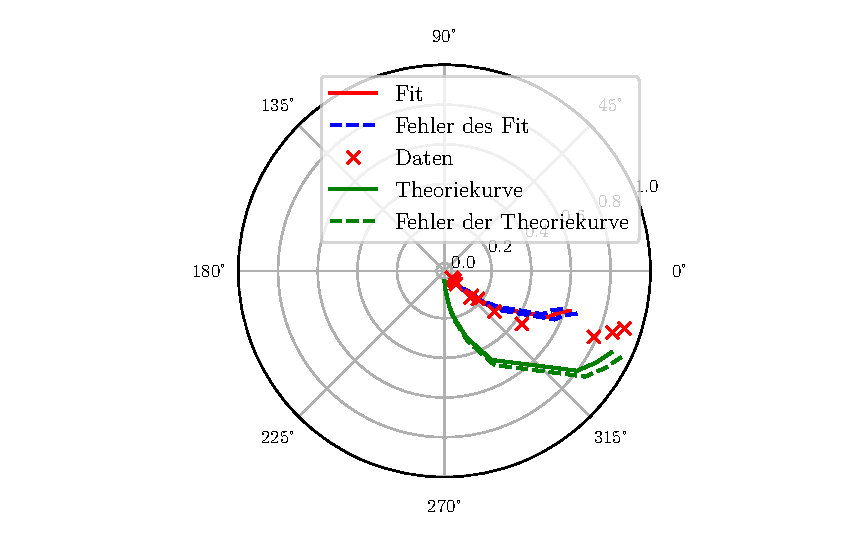
\includegraphics{build/plotd1.pdf}
  \caption{Plot}
  \label{fig:plotd1}
\end{figure}

\begin{figure}
  \centering
  \includegraphics{build/plotsd2.pdf}
  \caption{Plot}
  \label{fig:plotd2}
\end{figure}
\begin{figure}
  \centering
  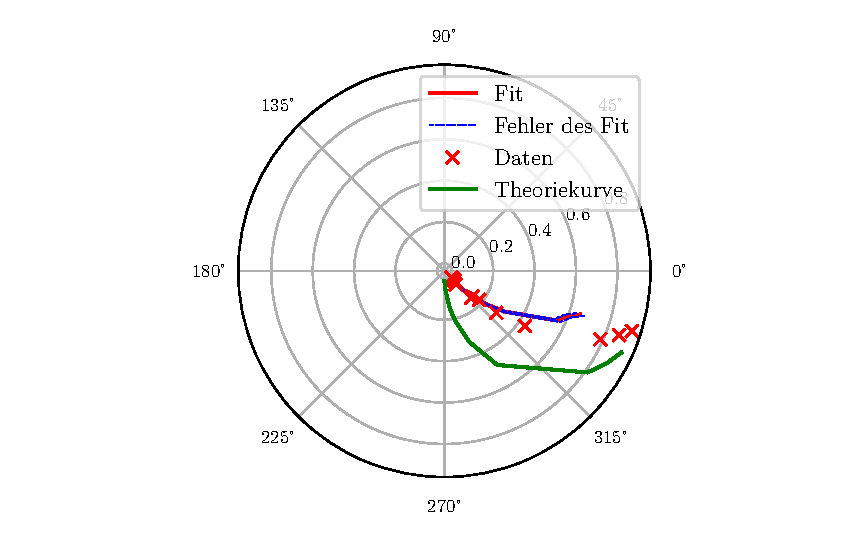
\includegraphics{build/plotd3.pdf}
  \caption{Plot}
  \label{fig:plotd3}
\end{figure}

%Integrator Bilder
\begin{figure}
  \centering
  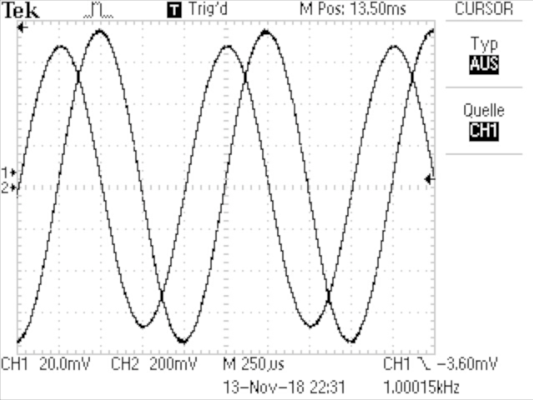
\includegraphics{build/integrator1.pdf}
  \caption{Plot}
  \label{fig:plot}
\end{figure}
\begin{figure}
  \centering
  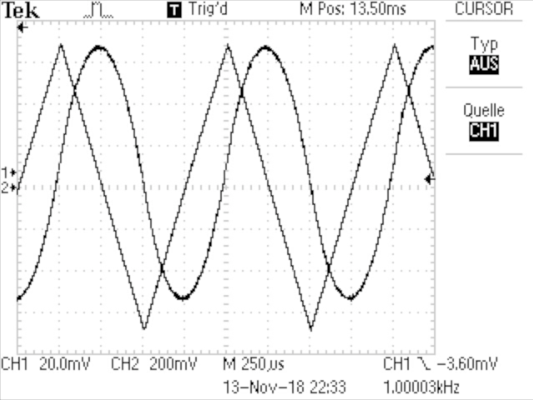
\includegraphics{build/integrator2.pdf}
  \caption{Plot}
  \label{fig:plot}
\end{figure}
\begin{figure}
  \centering
  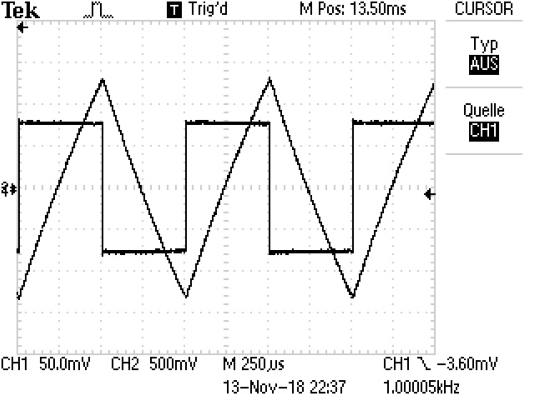
\includegraphics{build/integrator3.pdf}
  \label{fig:plot}
\end{figure}
%jeweils einzelne Formeln für RC in der Theorie angeben und hier erwähnen!
